\documentclass[12pt]{article}
\usepackage[utf8]{inputenc}
\usepackage{mathptmx,amsmath}
\usepackage{color}
\usepackage{listings}
\usepackage{setspace}
\usepackage{placeins}
\usepackage{graphicx}
\usepackage{geometry}
\usepackage{accsupp}
\renewcommand{\thelstnumber}{% Line number printing mechanism
  \protect\BeginAccSupp{ActualText={}}\arabic{lstnumber}\protect\EndAccSupp{}%
}
\geometry{margin=25mm}
\graphicspath{{images/}}
\definecolor{codegreen}{rgb}{0,0.6,0}
\definecolor{codegray}{rgb}{0.5,0.5,0.5}
\definecolor{codepurple}{rgb}{0.58,0,0.82}
\definecolor{codeblue}{rgb}{0,0,1}
\definecolor{codeblack}{rgb}{0,0,0}
\definecolor{Background}{rgb}{0.95,0.95,0.95}
\lstdefinestyle{pythonstyle}{
	numberstyle=\ttfamily\scriptsize\color{codegray},
	numbers=left,									
	numbersep=1em,
	xleftmargin=1em,
	framextopmargin=2em,
	framexbottommargin=2em,
	showspaces=false,
	showtabs=false,
	showstringspaces=false,
	frame=l,
	columns=flexible,
	tabsize=4,
	% Basic
	basicstyle=\ttfamily\footnotesize\setstretch{1},
	backgroundcolor=\color{Background},
	% Comments
	commentstyle=\color{codegray}\slshape,
	% Strings
	stringstyle=\color{codegreen},
	morecomment=[s][\color{codegreen}]{"""}{"""},
	morecomment=[s][\color{codegreen}]{'''}{'''},
	% keywords
	morekeywords={as, np, plt},		
	keywordstyle={\color{codeblue}\bfseries},
}
\lstset{
	style=pythonstyle, 
	language=Python,
	breaklines=true
	}

\begin{document}

%%%% Title Page
\begin{titlepage}

\newcommand{\HRule}{\rule{\linewidth}{0.5mm}} 							% horizontal line and its thickness
\center 
 
% University
\textsc{\LARGE Boğaziçi University}\\[1cm]

% Document info
\textsc{\Large Nonlinear Models in Operations Research}\\[0.2cm]
\textsc{\large IE 440}\\[1cm] 						% Course Code
\HRule \\[0.8cm]
{ \huge \bfseries Homework 2}\\[0.7cm]				% Assignment
\HRule \\[2cm]
\large
\emph{Authors:}\\
 M. Akın Elden\\Yunus Emre Karataş\\Y. Harun Kıvrıl\\Sefa Kayraklık \\[1.5cm]										% Author info
{\large 4 November 2019}\\[5cm]

\includegraphics[width=0.9\textwidth]{Boun_logo.png}\\[1cm] 	% University logo
\vfill 
\end{titlepage}


\onehalfspacing
\section{Introduction}

The project is implemented using Python as the programming language. The given data are read by using \textit{pandas} package, they are handled with the package \textit{numpy}, and the graphs are plotted by using the package \textit{matplotlib}.

\textbf{The necessary matrices are formed:}
\begin{lstlisting}[style=pythonstyle]
import numpy as np
import pandas as pd
import matplotlib.pyplot as plt
import seaborn; seaborn.set() # Plot styling

coordinates = pd.read_csv('coordinates_2_.csv')
demands = pd.read_csv('demand_2_.csv')
costs = pd.read_csv('costs_2_.csv')

A = np.asarray(coordinates) #first column= index of customer, second and third column= coordinates
H = np.abs(np.asarray(demands)) #first column= index of customer, second column= demand
C = np.abs(np.asarray(costs))   ##first column= index of facility, "i"th columns= cost of transporting 1 unit to the customer point "i"
# Index columns are removed
A = A[:,1:]
H = H[:,1]
C = C[:,1:]  
\end{lstlisting}

\section{Squared Euclidean Distance Solution of Single Facility Problem}
The single facility problem is solved by using squared Euclidean distance as a distance measurement. The objective function given that $m^{th}$ facility is chosen is given in the following expression.
\begin{equation} 
    min f(x_1,x_2)=min \sum_{j=1}^{n}h_jc_{mj}d(x_m,a_j)
\end{equation}
\begin{equation*}
    \begin{split}
    &\textit{, where }\\
        h_j &: \textit{the demand of customer j} \\
        c_{mj} &: \textit{the cost of transporting 1 unit of product from facility m to customer j per unit distance}\\
        a_j &: (a_{1j} , a_{2j}) \textit{ the coordinates of customer j} \\
        d(x_m,a_j) &: \textit{squared Euclidean distance from customer j to facility m} \\
    \end{split}
\end{equation*}

When the $1^{st}$ order necessary conditions are applied, the following expression is obtained.
\begin{equation}
    x_k^*=\frac{\sum_jh_jc_{mj}a_{kj}}{\sum_jh_jc_{mj}} \textit{, } k=1,2
\end{equation}

As proved in the class, the $x_k^*$ gives the optimum solution since $f(x_1,x_2)$ is a convex function.

\textbf{The source code used to implement the method:}
\begin{lstlisting}[style=pythonstyle]
def squaredDistSolforSingle(H=[], A=[], C=[], m=41):
    # If there is no assigned customer to facility, assign random location
    if A.size == 0:
        return np.random.randint(10,30),np.random.randint(10,30)
    facility_m = C[m] #cost vector of facility m: cost of transporting 1 unit from facility m to customer points
                                     #np.multiply(H[:,1],facility_m ->> output : element wise multiplier of cost vector and demand values
                                     #np.dot(H[:,1], facility_m) ->> output: total cost of transportation of demand
                                     #np.multiply(np.multiply(H[:,1],facility_m),A[:,1]) ->> weighted average of coordinates   
    x_v1_star = (np.sum(np.multiply(np.multiply(H,facility_m),A[:,0]))/np.dot(H, facility_m))
    x_v2_star = (np.sum(np.multiply(np.multiply(H,facility_m),A[:,1]))/np.dot(H, facility_m))
    
    return x_v1_star, x_v2_star
\end{lstlisting}

\subsection{Finding the location of the Facility42}
The above code is used to find the location of the facility which is selected as the $42^{nd}$. 

\textbf{The source code used to find the Facility42 location:}
\begin{lstlisting}[style=pythonstyle]
plt.scatter(A[:, 0], A[:, 1], s=np.size(A,axis=0), label='customers')

m=41 # selected facility

x1, x2 = squaredDistSolforSingle(H,A,C,m)
plt.scatter(x1,x2, marker='^', s = 150, label='facility'+ str(m+1))
plt.legend()

plt.savefig("{0}.png".format('Facility' + str(m+1)))
 
# C[m,:]*H ->> cost for each consumer per unit distance
# np.sum((A-[x1,x2])**2, axis=1) ->> squared distances of each consumer to facility m
# objFuncValue ->> total of the multiplication of cost per dist and distances
objFuncValue = np.dot(C[m,:]*H,np.sum((A-[x1,x2])**2, axis=1))

x1, x2, objFuncValue

\end{lstlisting}

The resulting facility location, the customer coordinates, and the objective function value are given in the following Figure.
\begin{figure}[ht] 
    \centering
    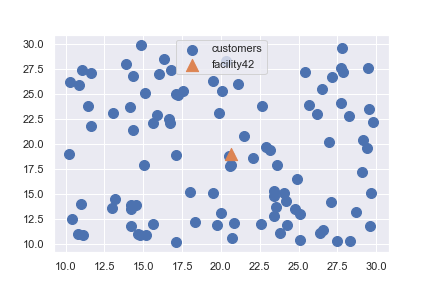
\includegraphics[height=25em]{Facility42.png}
    \caption{The graph of the locations of the consumers and Facilily42}
    \begin{center}
        \textit{$x^*=(20.62, 19.02), f(x^*)=344646.37$}
    \end{center}
\end{figure}
\FloatBarrier

\textbf{Conclusion:}\\
The location of the Facility42 is found as expected, since the middle point is likely to be selected as a facility location because it minimizes the average distances to the facility. And, the objective function value is the minimum value that can be obtained by using only the Facility42; however, it can be reduced by adding extra facilities, as this modification will be examined in the following sections.

\section{Euclidean Distance Solution of Single Facility Problem}
In this section the problem in Equation 1 is solved by taking $d(x_m,a_j)$  as \textit{Euclidean distance from customer j to facility m} \\. In order to solve this problem Weiszfeld Algorithim is implemented. For this problem it is known that Weiszfeld Algorithm converges to global minimum.

\textbf{The source code used to implement the method:}
\begin{lstlisting}[style=pythonstyle]
def Weiszfeld(H=[], A=[], C=[], m=41, eps = 0.001, print_iter = True):
    if A.size == 0:
        return np.random.randint(10,30),np.random.randint(10,30)
    cond = True
    itr = 0
    h = np.multiply(H, C[m])
    x_0 = (h @ A )/ np.sum(h)
    while cond:
        dj = np.sqrt(np.sum((A-x_0)**2, axis=1)) + eps
        x_1 = ((h / dj)  @ A) / np.sum((h / dj))
        cond = np.sqrt(np.sum((x_0-x_1)**2)) > eps
        x_0 = x_1
        itr += 1
    if print_iter:
        print('Total iterations: {0}'.format(itr))
    return x_1
\end{lstlisting}

\subsection{Finding the location of the Facility42}
The above code is used to find the location of the facility which is selected as the $42^{nd}$. 

\textbf{The source code used to find the Facility42 location:}
\begin{lstlisting}[style=pythonstyle]

x1, x2 = Weiszfeld(H,A,C,41)
obj = np.dot(C[m,:]*H,np.sum(np.sqrt((A-[x1,x2])**2), axis=1))
plt.scatter(A[:, 0], A[:, 1], s=np.size(A,axis=0), label = "consumers")
plt.scatter(x1,x2, marker='^', s = 150, label='facility'+ str(m+1))
plt.legend()
plt.savefig("{0}.png".format('Facility' + str(m+1)))

x1, x2, obj
\end{lstlisting}

The resulting facility location, the customer coordinates, and the objective function value are given in the following Figure.
\begin{figure}[ht] 
    \centering
    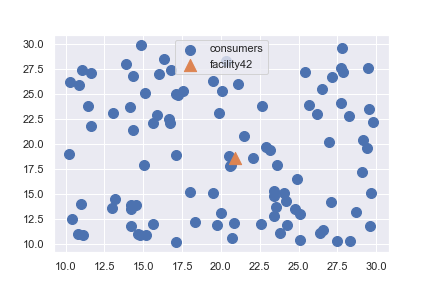
\includegraphics[height=25em]{EucFacility42.png}
    \caption{The graph of the locations of the consumers and Facility42}
    \begin{center}
        \textit{$x^*= (20.92, 18.68), f(x^*)=50708.21$}
    \end{center}
\end{figure}
\FloatBarrier

\textbf{Conclusion:}\\
The optimal facility location is close to the values found in squared Euclidean distance problem, so the result of the algorithm makes sense for us. The objective value is much less than the squared Euclidean case due to the taking an extra square root in the distance calculation. The location denoted by triangle in figure is the optimal solution that minimizes total the Euclidean distance to all customers.


\section{ALA Heuristic with Squared Euclidean Distance for Multi-Facility Weber Problem}

Multi facility problem is solved by using squared Euclidean distance as a distance measurement. In the ALA heuristic algorithm, initially customers are allocated to facilities randomly. If a facility is not assigned to a customer, it's location is determined randomly. After that each facility is located using squared Euclidean solution for single facility problem and new objective value is calculated. After that customers are allocated to the nearest facilities and then the facilities are located again. These allocation and location operations are performed iteratively until objective value (total cost value) stops decreasing. The objective function is given in the following expression.

\begin{align*}
    min &f(x_1,x_2)=min \sum_{i=1}^{m}\sum_{j=1}^{n}h_jc_{ij}d(x_i,a_j)y_{ij} \\ 
    s.t. &\sum_{i=1}^{m}y_{ij}= 1       j=1,2,...,n\\
    &y_{ij}=0,1      i=1,2,..,m  j=1,2,..,n    
\end{align*}
\begin{equation*}
    \begin{split}
    &\textit{, where }\\
        h_j &: \textit{the demand of customer j} \\
        c_{ij} &: \textit{the cost of transporting 1 unit of product from facility i to customer j per unit distance}\\
        a_j &: (a_{1j} , a_{2j}) \textit{ the coordinates of customer j} \\
        d(x_i,a_j) &: \textit{squared Euclidean distance from customer j to facility i} \\
        y_{ij} &: \textit{whether the facility i is assigned to customer j or not}
    \end{split}
\end{equation*}

\textbf{The source code used to implement the method:}
\begin{lstlisting}[style=pythonstyle]
def ALAHeuristicsSquaredEuclidean(H=[], A=[], C=[], seed=440): 
    cost_matrix = np.copy(C)
    m = np.size(C,0) # number of facilities
    n = np.size(C,1) # number of customers
    for i in range(n):
        cost_matrix[:,i] = H[i]*C[:,i]
    # Initial step, random assignments of customers
    facility_customers = [[] for i in range(m)]
    facility_locations = np.zeros(shape=(m,2))
    np.random.seed(seed)
    customer_assignments = np.array([np.random.randint(0,m) for i in range(n)])
    # Each customer is assigned to a facility randomly
    for i in range(n):
        facility_customers[customer_assignments[i]].append(i)
    # Solving m single facility location problems and computing new objective value until no improvement
    old_objective = np.iinfo(np.int32).max
    count = 0
    while(True):
        count += 1
        new_objective = 0
        for i in range(m):
            # Single facility for squared euclidean distance
            x1, x2 = squaredDistSolforSingle(H[facility_customers[i]],A[facility_customers[i]],C[:,facility_customers[i]],i)
            facility_locations[i] = np.array([x1,x2])
        # Calculating total cost between each facility and customer
        total_cost_matrix = np.zeros((n,m))
        for i in range(n):
            coord_dif_matrix = facility_locations - A[i]
            # for squared euclidean distance
            distance_matrix = np.sum(coord_dif_matrix**2, axis=1)
            total_cost_matrix[i] = np.transpose(cost_matrix[:,i])*distance_matrix
        # New objective value calculation
        for i in range(m):
            facility_cost = np.sum(total_cost_matrix[facility_customers[i],i])
            new_objective += facility_cost
        print('New objective: {0}'.format(new_objective))    
        if(new_objective>=old_objective):
            break
        old_objective = new_objective
        # Reassignment of customers according to distance to facilities
        facility_customers = [[] for i in range(m)]
        for i in range(n):
            nearest_facility = np.argmin(total_cost_matrix[i]) # index of minimum value
            facility_customers[nearest_facility].append(i)   
    print("Iteration number: {0}".format(count))    
    return facility_locations, facility_customers, new_objective
\end{lstlisting}

\subsection{Finding the location of the facilities}
The below code is used to find the location of the facilities:

\begin{lstlisting}[style=pythonstyle]
locations, assigned_customers, objective =ALAHeuristicsSquaredEuclidean(H,A,C)
#New objective: 174262.3093120177
#New objective: 4133.462783484186
#New objective: 2903.7097205835853
#New objective: 2503.0120264184566
#New objective: 1895.5898458663469
#New objective: 1736.1080485120947
#New objective: 1608.0409325073206
#New objective: 1608.0409325073206
#Iteration number: 8
\end{lstlisting}

The below code is used to draw each of the facilities with assigned customers:
\begin{lstlisting}[style=pythonstyle]
fig = plt.figure(figsize=(15,20))
for i in range(50):
    plt.title("Facility "+str(i))
    plt.subplot(10,5,i+1)
    plt.scatter(locations[i,0], locations[i,1], marker='^',c='r', s=60)
    plt.scatter(A[assigned_customers[i],0], A[assigned_customers[i],1],s=20)
    plt.tight_layout()
\end{lstlisting}

The resulting facility location and assigned customer coordinates are given in the following Figure.
\begin{figure}[ht] 
    \centering
    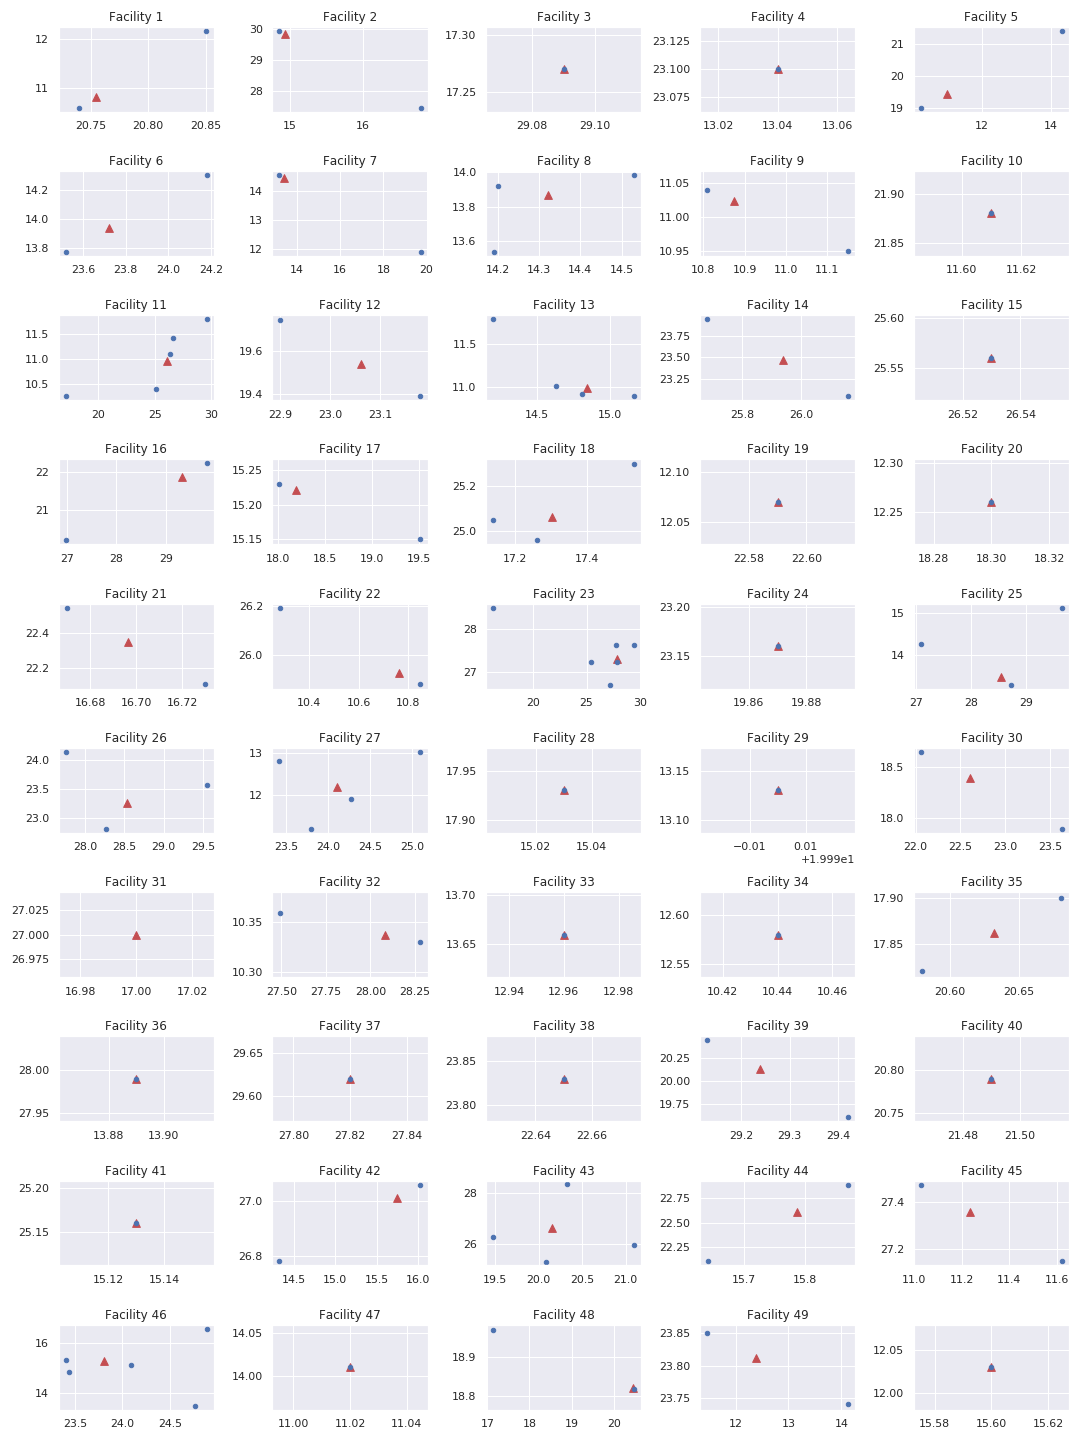
\includegraphics[width=\textwidth]{ala_squared_1.png}
    \caption{The graph of the locations of the consumers and facilities}
\end{figure}
\FloatBarrier
When all facilities and customers are drawn together in a plot, following figure occurs:
\begin{lstlisting}[style=pythonstyle]
plt.scatter(locations[:,0], locations[:,1], marker='^',c='r', s=60)
plt.scatter(A[:,0], A[:,1],s=20)
\end{lstlisting}
\begin{figure}[ht] 
    \centering
    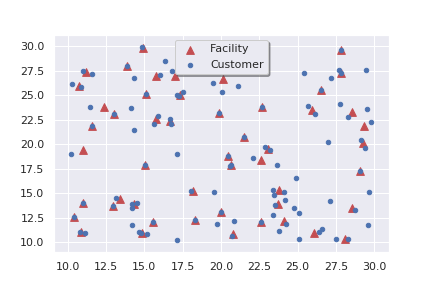
\includegraphics[height=25em]{ala_squared_2.png}
    \caption{The graph of the locations of the consumers and facilities}
\end{figure}

\begin{table}[h]
    
    \begin{minipage}{.49\linewidth}
    \begin{tabular}{|c|ccc|}
    \hline
    Facility & \textit{V1} & \textit{V2} & \textit{Assigned Custormers} \\
    \hline
1 & 20.75 & 10.82 &  36, 69          \\
2 & 14.93 & 29.86 &  31, 77          \\
3 & 29.09 & 17.27 &  45            \\
4 & 13.04 & 23.1 &  20            \\
5 & 10.99 & 19.44 &  17, 37          \\
6 & 23.72 & 13.93 &  30, 94          \\
7 & 13.41 & 14.46 &  23, 98          \\
8 & 14.32 & 13.87 &   6, 19, 96        \\
9 & 10.87 & 11.02 &  15, 58          \\
10 & 11.61 & 21.88 &  51            \\
11 & 26.06 & 10.96 &   5, 10, 29, 43, 63    \\
12 & 23.06 & 19.54 &   1, 82          \\
13 & 14.84 & 10.99 &   9, 35, 79, 84      \\
14 & 25.94 & 23.46 &  64, 74          \\
15 & 26.53 & 25.56 &  12            \\
16 & 29.31 & 21.87 &  72, 85          \\
17 & 18.2 & 15.22 &  22, 27          \\
18 & 17.3 & 25.06 &   4, 18, 89        \\
19 & 22.59 & 12.07 &  62            \\
20 & 18.3 & 12.26 &  95            \\
21 & 16.7 & 22.35 &  16,  46          \\
22 & 10.76 & 25.93 &  55,  56          \\
23 & 27.79 & 27.3 &   0,   3, 40, 70, 88, 91  \\
24 & 19.87 & 23.16 &  75            \\
25 & 28.54 & 13.47 &  21,  25, 76        \\
        \hline
    \end{tabular}
    \end{minipage}
     \begin{minipage}{.49\linewidth}
    \begin{tabular}{c|ccc|}
    \hline
    Facility & \textit{V1} & \textit{V2} & \textit{Assigned Custormers} \\
    \hline
26 & 28.53 & 23.26 &  14,  26, 68        \\
27 & 24.11 & 12.17 &  13,  28, 60, 67      \\
28 & 15.03 & 17.93 &  52            \\
29 & 19.99 & 13.13 &  93            \\
30 & 22.6 & 18.39 &   2,  24          \\
31 & 17 & 27 &             \\
32 & 28.08 & 10.34 &  34,  71          \\
33 & 12.96 & 13.66 &  48            \\
34 & 10.44 & 12.58 &  66            \\
35 & 20.63 & 17.86 &  33,  86          \\
36 & 13.89 & 27.99 &   8            \\
37 & 27.82 & 29.62 &  32            \\
38 & 22.65 & 23.83 &  59            \\
39 & 29.24 & 20.13 &  44,  81          \\
40 & 21.49 & 20.79 &  87            \\
41 & 15.13 & 25.16 &  90            \\
42 & 15.74 & 27.01 &  38,  41          \\
43 & 20.15 & 26.64 &  39,  42, 47 ,99      \\
44 & 15.79 & 22.61 &  57,  73          \\
45 & 11.24 & 27.36 &  53,  97          \\
46 & 23.81 & 15.31 &  50,  54, 65, 83, 92    \\
47 & 11.02 & 14.01 &  61            \\
48 & 20.45 & 18.82 &  11,  49          \\
49 & 12.39 & 23.81 &   7,  78          \\
50 & 15.6 & 12.03 &  80            \\

    \hline
    \end{tabular}
    \end{minipage}
\end{table}

\subsubsection*{Results with Different Seeds}
\begin{lstlisting}[style=pythonstyle]
ALAHeuristicsSquaredEuclidean(H,A,C, seed=300)
# New objective: 164251.16030488617
# New objective: 6093.684113289859
# New objective: 3339.4723444965266
# New objective: 2849.4433910221155
# New objective: 2795.1409238334118
# New objective: 2795.1409238334118
# Iteration number: 6

ALAHeuristicsSquaredEuclidean(H,A,C, seed=150)
# New objective: 186900.36366989513
# New objective: 5933.390226040791
# New objective: 3095.550353313043
# New objective: 2477.474936597154
# New objective: 2166.7345024250544
# New objective: 2052.876106989571
# New objective: 2052.876106989571
# Iteration number: 7

ALAHeuristicsSquaredEuclidean(H,A,C, seed=1001)
# New objective: 190499.69716511868
# New objective: 7924.693761385
# New objective: 4122.318794253405
# New objective: 3419.1384747910424
# New objective: 3260.7515102793936
# New objective: 3137.006364853382
# New objective: 2832.1403136836016
# New objective: 2782.0341933835666
# New objective: 2782.0341933835666
# Iteration number: 9
\end{lstlisting}

\FloatBarrier
\textbf{Conclusion:}\\
Most of the facilities are located between two or more customers. Also some of the facilities are located on the same location with a customer since it's assigned to only one customer. There is also one facility that is not assigned to any customer. The objective value (total cost) decreases fast at the beginning and then it decreases slowly and finally stops decreasing. Since the algorithm uses random initial starting points, results may change a little when different seeds are used to initialize algorithm. As a consequence, the algorithm gives reasonably good results.

\section{ALA Heuristic with Euclidean Distance for Multi-Facility Weber Problem}

The same multi facility problem is solved and a very similar algorithm is used but instead of using squared euclidean distance, this time euclidean distance is used as distance measurement and Weiszfeld single facility location algorithm is used to find the location of the facilities.

\textbf{The source code used to implement the method:}
\begin{lstlisting}[style=pythonstyle]
def ALAHeuristicsEuclidean(H=[], A=[], C=[], seed=440): 
    cost_matrix = np.copy(C)
    m = np.size(C,0) # number of facilities
    n = np.size(C,1) # number of customers
    for i in range(n):
        cost_matrix[:,i] = H[i]*C[:,i]
    # Initial step, random assignments of customers
    facility_customers = [[] for i in range(m)]
    facility_locations = np.zeros(shape=(m,2))
    np.random.seed(seed)
    customer_assignments = np.array([np.random.randint(0,m) for i in range(n)])
    # Each customer is assigned to a facility randomly
    for i in range(n):
        facility_customers[customer_assignments[i]].append(i)
    # Solving m single facility location problems and computing new objective value until no improvement
    old_objective = np.iinfo(np.int32).max
    count = 0
    while(True):
        count += 1
        new_objective = 0
        for i in range(m):
            # Single facility for euclidean distance
            x1, x2 = Weiszfeld(H[facility_customers[i]],A[facility_customers[i]],C[:,facility_customers[i]],i, print_iter=False)
            facility_locations[i] = np.array([x1,x2])
        # Calculating total cost between each facility and customer
        total_cost_matrix = np.zeros((n,m))
        for i in range(n):
            coord_dif_matrix = facility_locations - A[i]
            # for euclidean distance
            distance_matrix = np.sqrt(np.sum(coord_dif_matrix**2, axis=1))
            total_cost_matrix[i] = np.transpose(cost_matrix[:,i])*distance_matrix
        # New objective value calculation
        for i in range(m):
            facility_cost = np.sum(total_cost_matrix[facility_customers[i],i])
            new_objective += facility_cost
        print('New objective: {0}'.format(new_objective))    
        if(new_objective>=old_objective):
            break
        old_objective = new_objective
        # Reassignment of customers according to distance to facilities
        facility_customers = [[] for i in range(m)]
        for i in range(n):
            nearest_facility = np.argmin(total_cost_matrix[i]) # index of minimum value
            facility_customers[nearest_facility].append(i)   
    print("Iteration number: {0}".format(count))    
    return facility_locations, facility_customers, new_objective
\end{lstlisting}

\subsection{Finding the location of the facilities}
The below code is used to find the location of the facilities:

\begin{lstlisting}[style=pythonstyle]
locations, assigned_customers, objective = ALAHeuristicsEuclidean(H,A,C)
# New objective: 21277.419180220593
# New objective: 1823.4366305052527
# New objective: 1737.1326392135893
# New objective: 1714.2142423187183
# New objective: 1569.7426767483316
# New objective: 1473.772282041133
# New objective: 1459.1965550516459
# New objective: 1371.4628545516036
# New objective: 1346.452365629547
# New objective: 1346.452365629547
# Iteration number: 10
\end{lstlisting}

The below code is used to draw each of the facilities with assigned customers:
\begin{lstlisting}[style=pythonstyle]
fig = plt.figure(figsize=(15,20))
for i in range(50):
    plt.title("Facility "+str(i))
    plt.subplot(10,5,i+1)
    plt.scatter(locations[i,0], locations[i,1], marker='^',c='r', s=60)
    plt.scatter(A[assigned_customers[i],0], A[assigned_customers[i],1],s=20)
    plt.tight_layout()
\end{lstlisting}

The resulting facility location and assigned customer coordinates are given in the following Figure.
\begin{figure}[ht] 
    \centering
    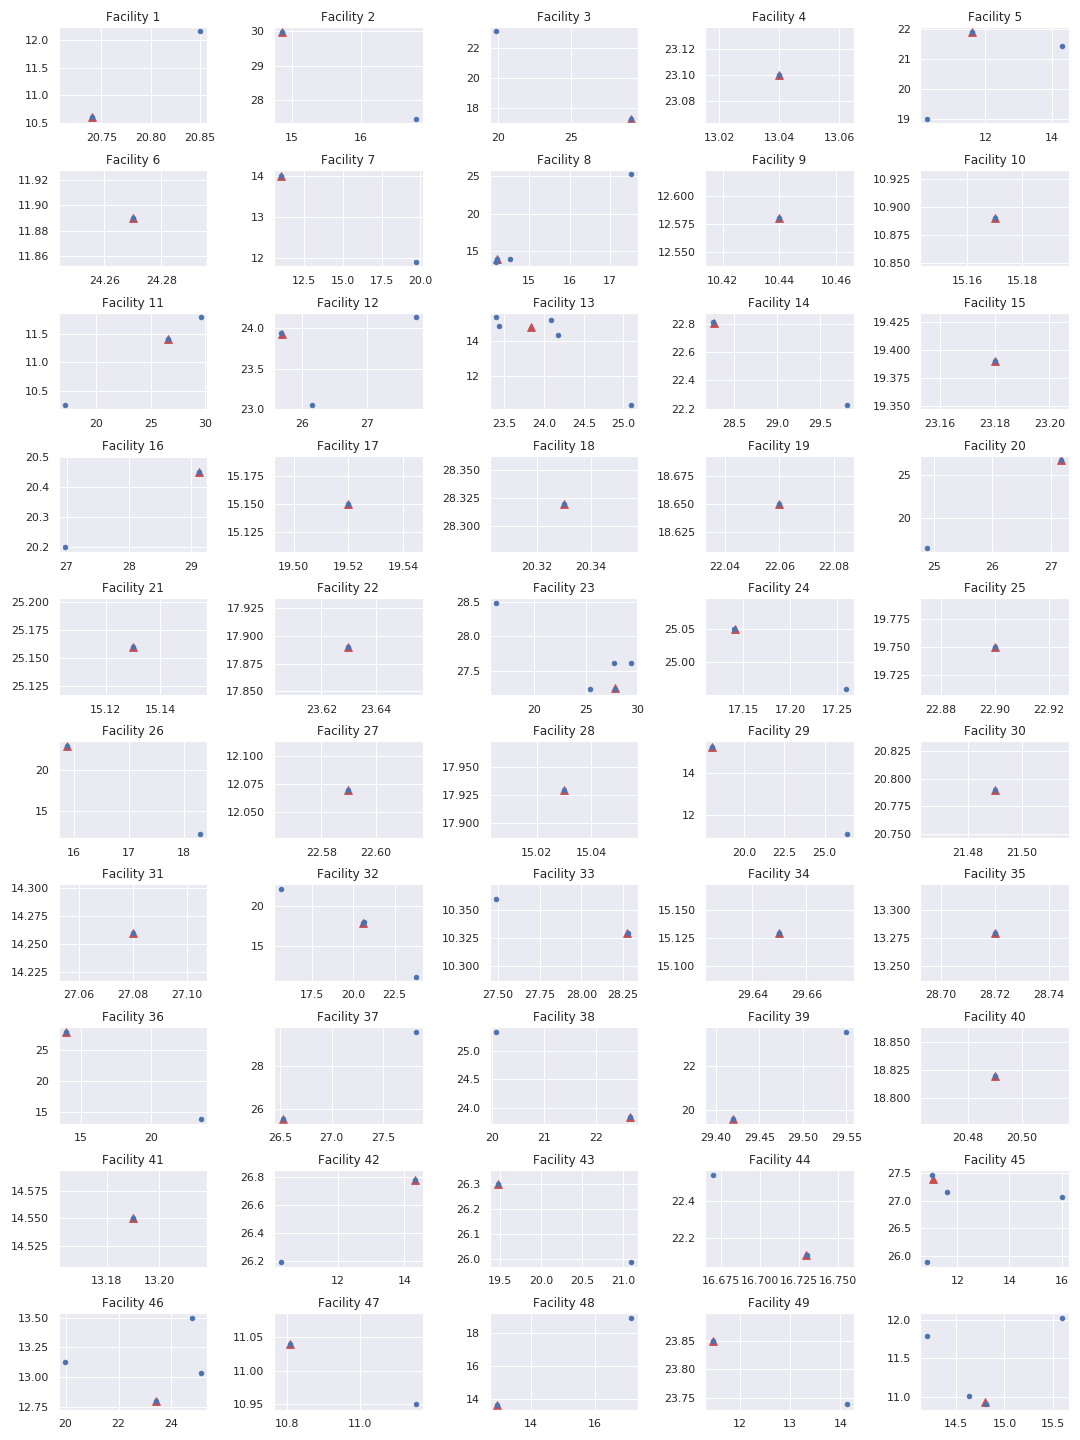
\includegraphics[width=\textwidth]{ala_euclidean_1.png}
    \caption{The graph of the locations of the consumers and facilities}
\end{figure}
\FloatBarrier
When all facilities and customers are drawn together in a plot, following figure occurs:
\begin{lstlisting}[style=pythonstyle]
plt.scatter(locations[:,0], locations[:,1], marker='^',c='r', s=60, label='Facility')
plt.scatter(A[:,0], A[:,1],s=20, label='Customer')
plt.legend(shadow=True)
\end{lstlisting}
\begin{figure}[ht] 
    \centering
    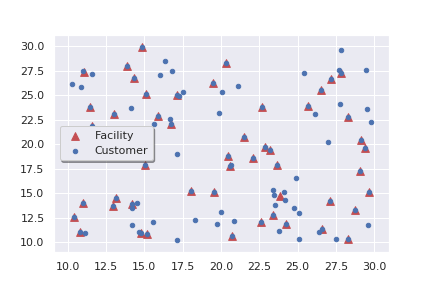
\includegraphics[height=25em]{ala_euclidean_2.png}
    \caption{The graph of the locations of the consumers and facilities}
\end{figure}

\begin{table}[h]
    
    \begin{minipage}{.49\linewidth}
    \begin{tabular}{|c|ccc|}
    \hline
    Facility & \textit{V1} & \textit{V2} & \textit{Assigned Custormers} \\
    \hline
1 & 20.74 & 10.61 &   36, 69  \\
2 & 14.86 & 29.96 &   31, 77  \\
3 & 29.09 & 17.27 &   45, 75  \\
4 & 13.04 & 23.1 &   20,   \\
5 & 11.61 & 21.88 &   17, 37, 51   \\
6 & 24.27 & 11.89 &   28     \\
7 & 11.02 & 14.01 &   23, 61  \\
8 & 14.21 & 13.92 &    4,  6, 19, 96  \\
9 & 10.44 & 12.58 &   66     \\
10 & 15.17 & 10.89 &   35     \\
11 & 26.6 & 11.41 &   10, 29, 63   \\
12 & 25.7 & 23.93 &   64, 68, 74   \\
13 & 23.83 & 14.75 &   43, 50, 65, 83,  94 \\
14 & 28.27 & 22.81 &   26, 85  \\
15 & 23.18 & 19.39 &   82     \\
16 & 29.13 & 20.45 &   44, 72  \\
17 & 19.52 & 15.15 &   27     \\
18 & 20.33 & 28.32 &   47     \\
19 & 22.06 & 18.65 &    2     \\
20 & 27.17 & 26.71 &    0, 92  \\
21 & 15.13 & 25.16 &   90     \\
22 & 23.63 & 17.89 &   24     \\
23 & 27.85 & 27.25 &    3, 40, 70, 88, 91 \\
24 & 17.14 & 25.05 &   18, 89  \\
25 & 22.9 & 19.75 &    1     \\
        \hline
    \end{tabular}
    \end{minipage}
     \begin{minipage}{.49\linewidth}
    \begin{tabular}{c|ccc|}
    \hline
    Facility & \textit{V1} & \textit{V2} & \textit{Assigned Custormers} \\
    \hline
26 & 15.87 & 22.89 &   73, 95  \\
27 & 22.59 & 12.07 &   62     \\
28 & 15.03 & 17.93 &   52     \\
29 & 18.02 & 15.23 &    5, 22  \\
30 & 21.49 & 20.79 &   87     \\
31 & 27.08 & 14.26 &   25     \\
32 & 20.6 & 17.83 &   33, 57, 67, 86  \\
33 & 28.28 & 10.33 &   34, 71,  \\
34 & 29.65 & 15.13 &   76     \\
35 & 28.72 & 13.28 &   21     \\
36 & 13.89 & 27.99 &    8, 30  \\
37 & 26.53 & 25.56 &   12, 32  \\
38 & 22.65 & 23.83 &   59, 99  \\
39 & 29.42 & 19.6 &   14, 81  \\
40 & 20.49 & 18.82 &   11     \\
41 & 13.19 & 14.55 &   98     \\
42 & 14.33 & 26.78 &   38, 55  \\
43 & 19.48 & 26.3 &   39, 42  \\
44 & 16.73 & 22.11 &   16, 46  \\
45 & 11.08 & 27.39 &   41, 53, 56,  97  \\
46 & 23.42 & 12.8 &   13, 54, 60,  93  \\
47 & 10.81 & 11.04 &   15, 58  \\
48 & 12.96 & 13.66 &   48, 49  \\
49 & 11.46 & 23.85 &    7, 78  \\
50 & 14.8 & 10.93 &    9, 79, 80,  84  \\
    \hline
    \end{tabular}
    \end{minipage}
\end{table}
\FloatBarrier

\subsubsection*{Results with Different Seeds}
\begin{lstlisting}[style=pythonstyle]
ALAHeuristicsEuclidean(H,A,C, seed=300)
# New objective: 20382.639116582784
# New objective: 1926.8155984587638
# New objective: 1470.3896888708512
# New objective: 1416.7542750664556
# New objective: 1379.2453610144432
# New objective: 1379.2453610144432
# Iteration number: 6

ALAHeuristicsEuclidean(H,A,C, seed=101)
# New objective: 20406.465353482425
# New objective: 2192.0738779233543
# New objective: 1864.8329223136586
# New objective: 1645.5789518304855
# New objective: 1645.5789518304855
# Iteration number: 5

ALAHeuristicsEuclidean(H,A,C, seed=1001)
# New objective: 23353.276620906207
# New objective: 2049.6213448391472
# New objective: 1782.1177795295437
# New objective: 1734.9743730241787
# New objective: 1590.9695283313324
# New objective: 1546.521090803287
# New objective: 1546.521090803287
# Iteration number: 7
\end{lstlisting}

\textbf{Conclusion:}\\
While ALA Heuristics gives centralized facilities with squared euclidean distance, when euclidean distance is used in ALA Heuristic facilities are tended to be located on a customer's location. The reason is that, since the costs are not equal and euclidean distance considers linear distance, moving away from the customer with lower cost and getting closer to the customer with higher cost always decreases the total cost in a two assigned customers case. But the common point is that, both of the algorithms gives a little different results with different seeds.

\section{Appendix}
The complete script file:
\begin{lstlisting}[style=pythonstyle,numbers=none]
import numpy as np
import pandas as pd
import matplotlib.pyplot as plt
import seaborn; seaborn.set() # Plot styling

coordinates = pd.read_csv('coordinates_2_.csv')
demands = pd.read_csv('demand_2_.csv')
costs = pd.read_csv('costs_2_.csv')

A = np.asarray(coordinates) #first column= index of customer, second and third column= coordinates
H = np.abs(np.asarray(demands)) #first column= index of customer, second column= demand
C = np.abs(np.asarray(costs))   ##first column= index of facility, "i"th columns= cost of transporting 1 unit to the customer point "i"
# index columns are removed
A = A[:,1:]
H = H[:,1]
C = C[:,1:]  

def squaredDistSolforSingle(H=[], A=[], C=[], m=41):
    # If there is no assigned customer to facility, assign random location
    if A.size == 0:
        return np.random.randint(10,30),np.random.randint(10,30)
    facility_m = C[m] #cost vector of facility m: cost of transporting 1 unit from facility m to customer points
                                     #np.multiply(H[:,1],facility_m ->> output : element wise multiplier of cost vector and demand values
                                     #np.dot(H[:,1], facility_m) ->> output: total cost of transportation of demand
                                     #np.multiply(np.multiply(H[:,1],facility_m),A[:,1]) ->> weighted average of coordinates   
    x_v1_star = (np.sum(np.multiply(np.multiply(H,facility_m),A[:,0]))/np.dot(H, facility_m))
    x_v2_star = (np.sum(np.multiply(np.multiply(H,facility_m),A[:,1]))/np.dot(H, facility_m))
    
    return x_v1_star, x_v2_star

plt.scatter(A[:, 0], A[:, 1], s=np.size(A,axis=0), label='consumers')

m=41 # selected facility

x1, x2 = squaredDistSolforSingle(H,A,C,m)

plt.scatter(x1,x2, marker='^', s = 150, label='facility'+ str(m+1))
plt.legend()
plt.savefig("{0}.png".format('Facility' + str(m+1)))

# C[m,:]*H ->> cost for each consumer per unit distance
# np.sum((A-[x1,x2])**2, axis=1) ->> squared distances of each consumer to facility m
# objFuncValue ->> total of the multiplication of cost per dist and distances
objFuncValue = np.dot(C[m,:]*H,np.sum((A-[x1,x2])**2, axis=1))

x1, x2, objFuncValue

def Weiszfeld(H=[], A=[], C=[], m=41, eps = 0.001, print_iter = True):
    if A.size == 0:
        return np.random.randint(10,30),np.random.randint(10,30)
    cond = True
    itr = 0
    h = np.multiply(H, C[m])
    x_0 = (h @ A )/ np.sum(h)
    while cond:
        dj = np.sqrt(np.sum((A-x_0)**2, axis=1)) + eps
        x_1 = ((h / dj)  @ A) / np.sum((h / dj))
        cond = np.sqrt(np.sum((x_0-x_1)**2)) > eps
        x_0 = x_1
        itr += 1
    if print_iter:
        print('Total iterations: {0}'.format(itr))
    return x_1


plt.scatter(A[:, 0], A[:, 1], s=np.size(A,axis=0), label = "consumers")

x1, x2 = Weiszfeld(H,A,C,41)

plt.scatter(x1,x2, marker='^', s = 150, label='facility'+ str(m+1))
plt.legend()
plt.savefig("{0}.png".format('EucFacility' + str(m+1)))

obj = np.dot(C[m,:]*H,np.sum(np.sqrt((A-[x1,x2])**2), axis=1))

x1, x2, obj

def ALAHeuristicsSquaredEuclidean(H=[], A=[], C=[], seed=440): 
    cost_matrix = np.copy(C)
    m = np.size(C,0) # number of facilities
    n = np.size(C,1) # number of customers
    for i in range(n):
        cost_matrix[:,i] = H[i]*C[:,i]
    # Initial step, random assignments of customers
    facility_customers = [[] for i in range(m)]
    facility_locations = np.zeros(shape=(m,2))
    np.random.seed(seed)
    customer_assignments = np.array([np.random.randint(0,m) for i in range(n)])
    # Each customer is assigned to a facility randomly
    for i in range(n):
        facility_customers[customer_assignments[i]].append(i)
    # Solving m single facility location problems and computing new objective value until no improvement
    old_objective = np.iinfo(np.int32).max
    count = 0
    while(True):
        count += 1
        new_objective = 0
        for i in range(m):
            # Single facility for squared euclidean distance
            x1, x2 = squaredDistSolforSingle(H[facility_customers[i]],A[facility_customers[i]],C[:,facility_customers[i]],i)
            facility_locations[i] = np.array([x1,x2])
        # Calculating total cost between each facility and customer
        total_cost_matrix = np.zeros((n,m))
        for i in range(n):
            coord_dif_matrix = facility_locations - A[i]
            # for squared euclidean distance
            distance_matrix = np.sum(coord_dif_matrix**2, axis=1)
            total_cost_matrix[i] = np.transpose(cost_matrix[:,i])*distance_matrix
        # New objective value calculation
        for i in range(m):
            facility_cost = np.sum(total_cost_matrix[facility_customers[i],i])
            new_objective += facility_cost
        print('New objective: {0}'.format(new_objective))    
        if(new_objective>=old_objective):
            break
        old_objective = new_objective
        # Reassignment of customers according to distance to facilities
        facility_customers = [[] for i in range(m)]
        for i in range(n):
            nearest_facility = np.argmin(total_cost_matrix[i]) # index of minimum value
            facility_customers[nearest_facility].append(i)   
    print("Iteration number: {0}".format(count))    
    return facility_locations, facility_customers, new_objective

locations, assigned_customers, objective =ALAHeuristicsSquaredEuclidean(H,A,C)

fig = plt.figure(figsize=(15,20))
for i in range(50):
    plt.title("Facility "+str(i))
    plt.subplot(10,5,i+1)
    plt.scatter(locations[i,0], locations[i,1], marker='^',c='r', s=60)
    plt.scatter(A[assigned_customers[i],0], A[assigned_customers[i],1],s=20)
    plt.tight_layout()
plt.savefig("ala_squared_1.png")


plt.scatter(locations[:,0], locations[:,1], marker='^',c='r', s=60, label='Facility')
plt.scatter(A[:,0], A[:,1],s=20, label='Customer')
plt.legend(shadow=True)
plt.savefig("ala_squared_2.png")

def ALAHeuristicsEuclidean(H=[], A=[], C=[], seed=440): 
    cost_matrix = np.copy(C)
    m = np.size(C,0) # number of facilities
    n = np.size(C,1) # number of customers
    for i in range(n):
        cost_matrix[:,i] = H[i]*C[:,i]
    # Initial step, random assignments of customers
    facility_customers = [[] for i in range(m)]
    facility_locations = np.zeros(shape=(m,2))
    np.random.seed(seed)
    customer_assignments = np.array([np.random.randint(0,m) for i in range(n)])
    # Each customer is assigned to a facility randomly
    for i in range(n):
        facility_customers[customer_assignments[i]].append(i)
    # Solving m single facility location problems and computing new objective value until no improvement
    old_objective = np.iinfo(np.int32).max
    count = 0
    while(True):
        count += 1
        new_objective = 0
        for i in range(m):
            # Single facility for euclidean distance
            x1, x2 = Weiszfeld(H[facility_customers[i]],A[facility_customers[i]],C[:,facility_customers[i]],i, print_iter=False)
            facility_locations[i] = np.array([x1,x2])
        # Calculating total cost between each facility and customer
        total_cost_matrix = np.zeros((n,m))
        for i in range(n):
            coord_dif_matrix = facility_locations - A[i]
            # for euclidean distance
            distance_matrix = np.sqrt(np.sum(coord_dif_matrix**2, axis=1))
            total_cost_matrix[i] = np.transpose(cost_matrix[:,i])*distance_matrix
        # New objective value calculation
        for i in range(m):
            facility_cost = np.sum(total_cost_matrix[facility_customers[i],i])
            new_objective += facility_cost
        print('New objective: {0}'.format(new_objective))    
        if(new_objective>=old_objective):
            break
        old_objective = new_objective
        # Reassignment of customers according to distance to facilities
        facility_customers = [[] for i in range(m)]
        for i in range(n):
            nearest_facility = np.argmin(total_cost_matrix[i]) # index of minimum value
            facility_customers[nearest_facility].append(i)   
    print("Iteration number: {0}".format(count))    
    return facility_locations, facility_customers, new_objective

locations, assigned_customers, objective =ALAHeuristicsEuclidean(H,A,C)

fig = plt.figure(figsize=(15,20))
for i in range(50):
    plt.title("Facility "+str(i))
    plt.subplot(10,5,i+1)
    plt.scatter(locations[i,0], locations[i,1], marker='^',c='r', s=60)
    plt.scatter(A[assigned_customers[i],0], A[assigned_customers[i],1],s=20)
    plt.tight_layout()
plt.savefig("ala_euclidean_1.png")


plt.scatter(locations[:,0], locations[:,1], marker='^',c='r', s=60, label='Facility')
plt.scatter(A[:,0], A[:,1],s=20, label='Customer')
plt.legend(shadow=True)
plt.savefig("ala_euclidean_2.png")

\end{lstlisting}

\end{document}
